\chapter{実験方法}
\section{概要}
本実験では,0.5,1wt.\% ポリアクリルアミド(PAA)溶液(三菱ケミカル,AP805C)を擬塑性流体としてそれぞれ用いた.また,対照実験として水道水も用いた.作製したPAA溶液が適切なものであるか評価を行うため,非ニュートン流体における指標の一つとなる粘度の計測を行った.続いて,擬塑性流体に対する超音波照射による影響の密度依存性を調べるため,様々な落下球を用いて球落下実験行った.

\section{粘度計測}
粘度計測における計測機器の模式図をFig.\ref{fig:viscosity}に示す.ステージと回転する円錐回転子の間に存在する試料によって付加されるトルクを計測することで粘度の計測を行う.粘度のせん断速度依存性を確認することで生成した溶液の性質の確認を行った.なお、計測範囲の都合上、水道水では1°34′×R24のコーンロータを,PAA溶液では1°34′×R12のコーンロータをそれぞれ用いた.

\begin{table}[h]
    \centering
    \caption{Specifications of viscometer(東機産業,TVE-25L)}
    \label{table:viscometer}
    \begin{tabular}{c|c}\hline
        測定方式    & 円錐平板方式                    \\ \hline
        回転速度    & 0,0.1~100.0rpm;0.1rpmステップ \\ \hline
        精度/再現性 & \begin{tabular}{c}
            フルスケールの±1.0\%以内/ \\
            フルスケールの±0.2\%以内
        \end{tabular}       \\ \hline
    \end{tabular}
\end{table}
\begin{center}
    \begin{figure}[H]
        \centering
        \includegraphics[clip,width=8.0cm]{2-Methods/Viscosity-Measurement.png}
        \caption{Viscosity measurement method.}
        \label{fig:viscosity}
    \end{figure}
\end{center}

\section{圧力場の測定}

圧力場測定の概略図を\ref{fig:microphone}に示す.圧力測定にはハイドロフォン(Br\"{u}el \& Kj\ae r,Hydrophone Type8103)を用いた.ハイドロフォンの出力電圧をコンディショニングアンプ(Br\"{u}el \& Kj\ae r,NEXUS Change Amplifier Type 2692-A-0S1)を用いて増幅し,オシロスコープを用いて電圧を記録した.記録した電圧より,コンディショニングアンプの設定を電圧を圧力場に変換した.

\begin{table}[ht]
    \centering
    \caption{Specifications of microphone (Br\"{u}el \& Kj\ae r,Hydrophone Type8103)}
    \label{table:microphone}
    \begin{tabular}{c|c}\hline
        公称電圧感度 & 29$\mu$V/Pa   \\ \hline
        計測範囲     & 0.1kHz-180kHz \\ \hline
    \end{tabular}
\end{table}

\begin{table}[ht]
    \centering
    \caption{Specifications of conditioning amplifier(Br\"{u}el \& Kj\ae r,NEXUS Change Amplifier Type 2692-A-0S1)}
    \label{table:conditioning amplifier}
    \begin{tabular}{c|c}\hline
        マイクロフォン入力 &                                   \\ \hline
        入力インピーダンス & 10M$\Omega$\textbar \textbar300pF \\ \hline
        最大入力           & 31.6V                             \\ \hline
        周波数範囲(-1dB) & 0.1kHz-100kHz(ゲイン$\leq$60dB)   \\ \hline
    \end{tabular}
\end{table}

\begin{center}
    \begin{figure}[ht]
        \centering
        \label{fig:microphone}
        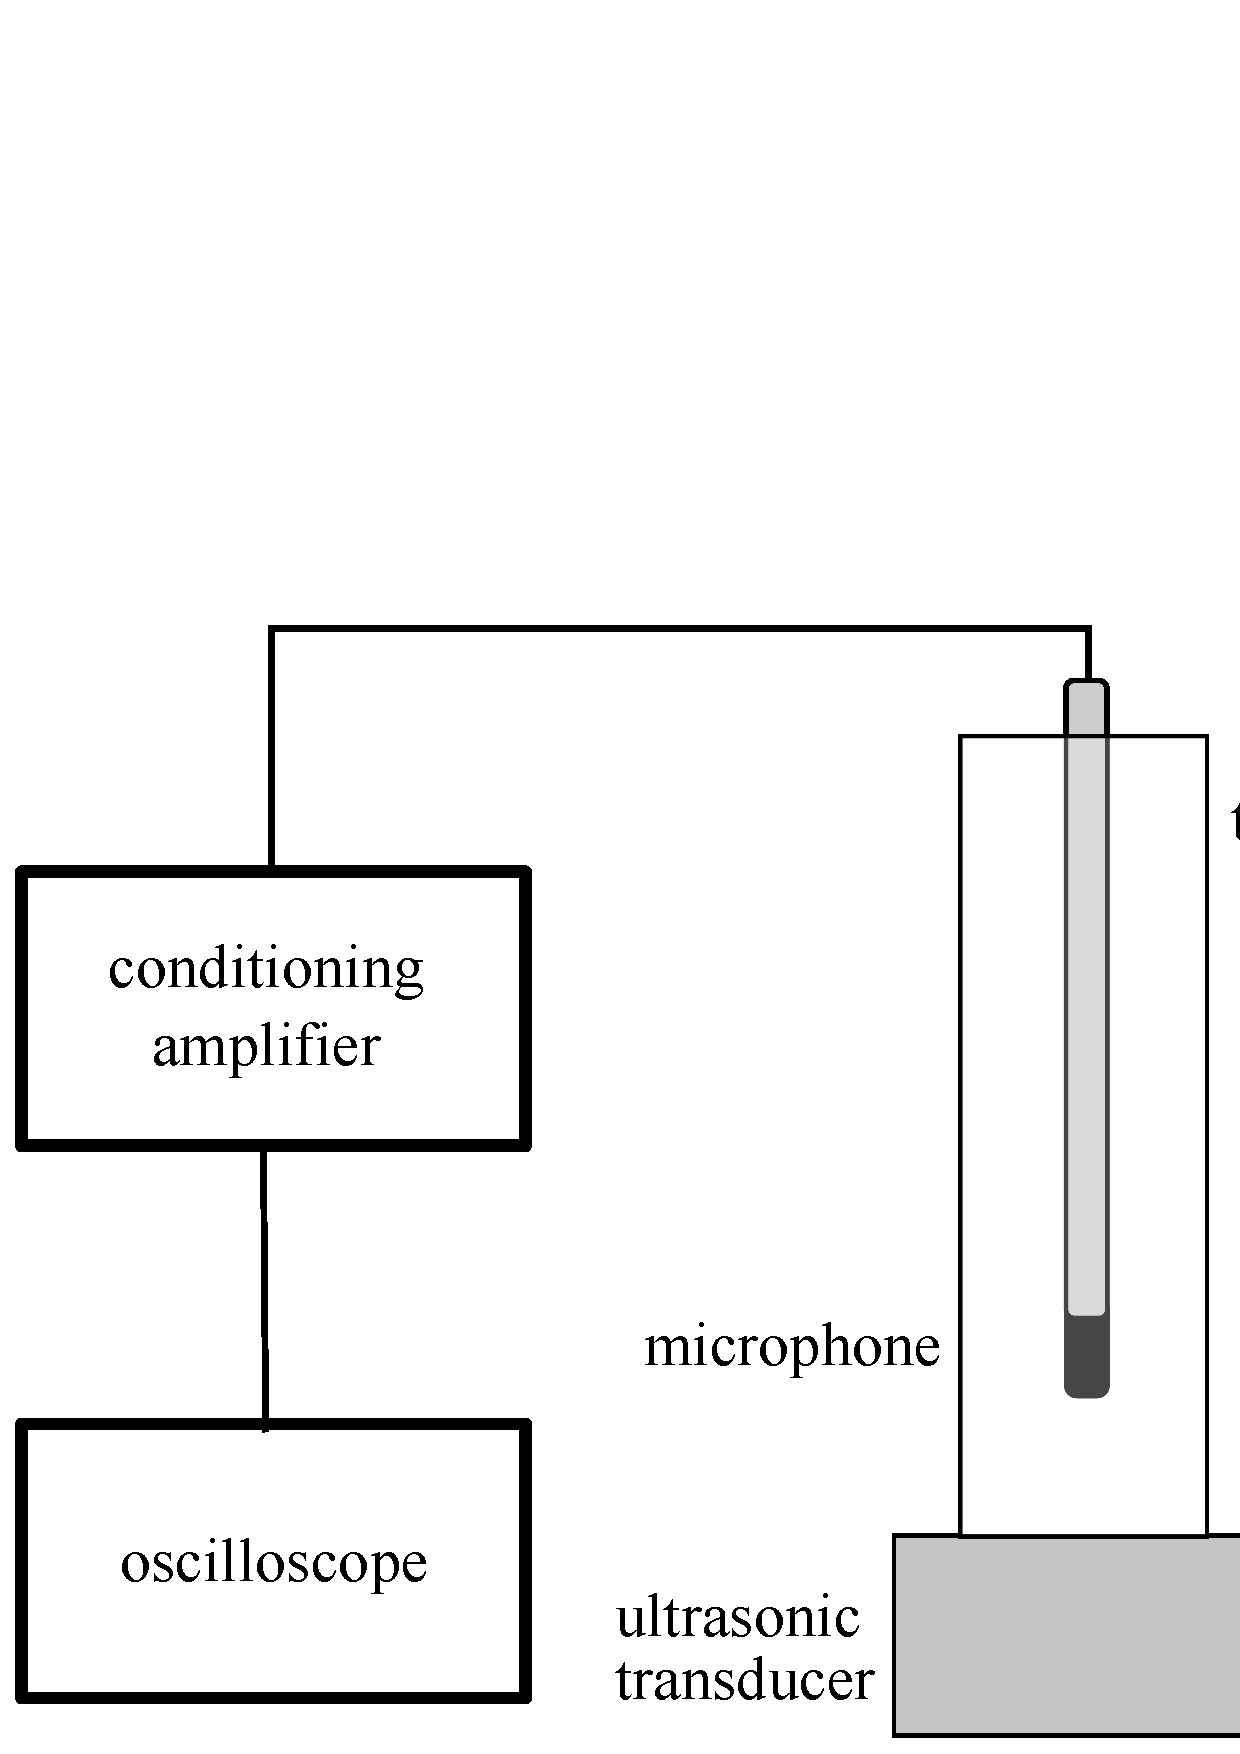
\includegraphics[clip,width=8.0cm]{2-Methods/microphone.png}
        \caption{Schematic outline for pressure measurement.}
    \end{figure}
\end{center}

\section{球落下実験}

使用した実験装置の概略図をFig.\ref{fig:device}に示す.外寸において高さ255mm,幅50mm,奥行き50mm,厚さ5mmの矩形アクリル水槽に試験溶液を満たした.その上に落下球把持用のピックアップツールをマグネットベースによって固定した.そのピックアップツールを用いて落下球の保持した.ピックアップツールによる把持を解除することにより,球の保持を解除した.落下球の直径はD=10mmのものを用いた.落下球が試験液体中を落下する様子をハイスピードカメラ(BASLER, acA1920-150um)で撮影し,記録用コンピュータに連続画像(bmp形式)として保存した.ハイスピードカメラにはレンズ(BASLER, TS5014-MP)をつけ,絞り,焦点の調整を行い,明瞭に鋼球を撮影できるようにした.実験装置後方にスクリーン,赤外線ライトを設置し,装置を後方より照射することにより,落下の様子をより分かりやすくした.さらに,超音波振動による影響を調査するためにアクリル水槽の下に超音波振動子を設置した.

\begin{table}[ht]
    \centering
    \caption{Specifications of high-speed camera (BASLER, acA1920-150um)}
    \label{table:camera}
    \begin{tabular}{c|c}\hline
        センサ種別      & CMOS                \\ \hline
        水平/垂直解像度 & 320px$\times$1264px \\ \hline
        解像度          & 0.4MP               \\ \hline
        フレームレート  & 210fps              \\ \hline
    \end{tabular}
\end{table}

\begin{table}[ht]
    \centering
    \caption{Specifications of lens (BASLER, TS5014-MP)}
    \label{table:lens}
    \begin{tabular}{c|c}\hline
        焦点距離[mm]     & 50.0     \\ \hline
        F値              & 1.4-16.0 \\ \hline
        最短撮影距離[mm] & 500      \\ \hline
    \end{tabular}
\end{table}

\begin{figure}[ht]
    \centering
    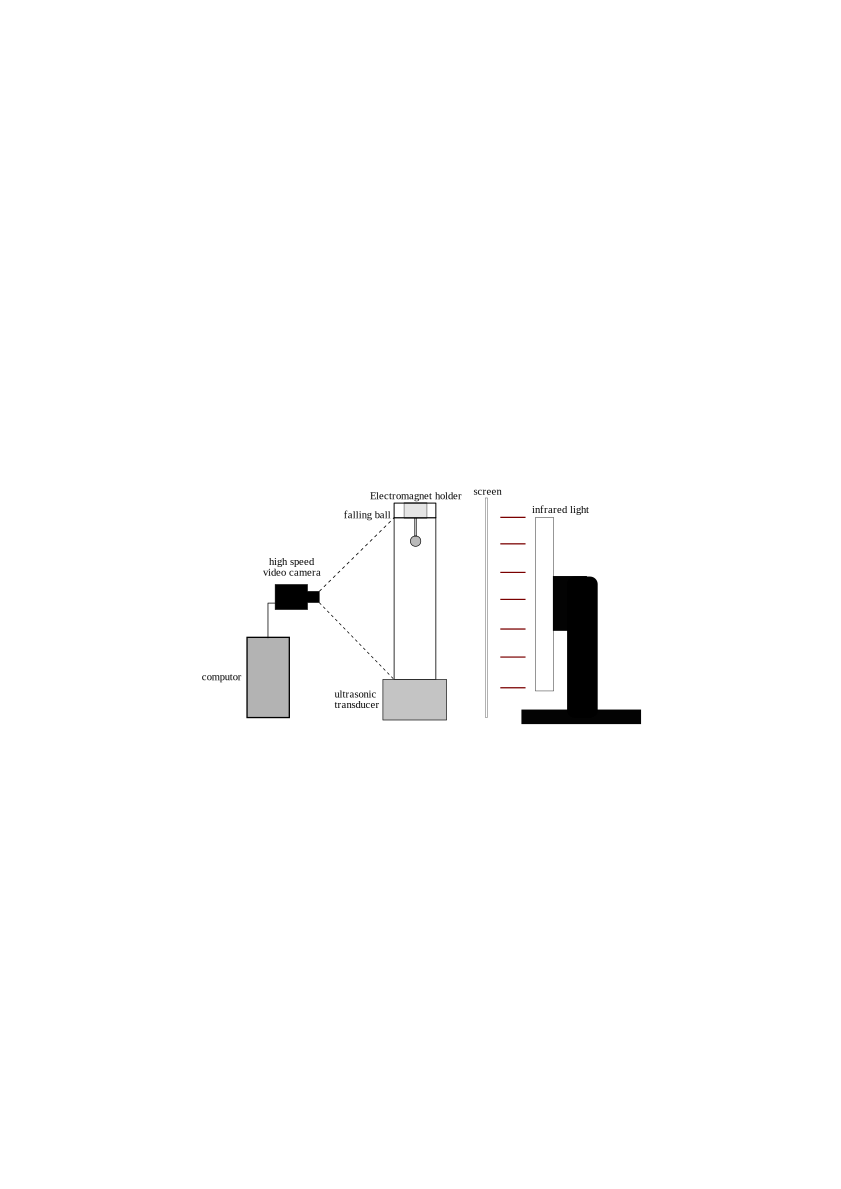
\includegraphics[clip,width=15.0cm]{2-Methods/device.png}
    \caption{Schematic view of the experimental apparatus.}
    \label{fig:device}
\end{figure}

超音波振動子の発振には,ファンクションジェネレータ(NF,WF1974),オシロスコープ(IWATSU,DIGITAL OSCILLOSCOPE DS-5614A),パワーアンプ(NF,HSA4101)を用いた.これらの接続をFig.\ref{fig:connect-with-signal}に示す.ファンクションジェネレータによって,周波数,電圧の制御を行い,超音波出力の出力元となる正弦波信号を生成した.続いて,ファンクションジェネレータによって生成された正弦波信号をパワーアンプによって,20倍のゲインをかけ増幅した.これら,オシロスコープによってファンクションジェネレータによって生成された信号,パワーアンプによって増幅された信号の両方をモニタリングし正常に出力されているか確認を行った.また,パワーアンプによって増幅された信号を,ランジュバン型振動子(富士セラミックス,FBL28502HA)上に円形のSUS304製プレートを接着したものを振動子とした.超音波振動子の共振周波数は28kHzである.

\begin{figure}[ht]
    \centering
    \includegraphics[clip,width=15.0cm]{2-Methods/connect-with-signal.png}
    \caption{How to connect with signal generator and ultrasonic transducers.}
    \label{fig:connect-with-signal}
\end{figure}

\section{実験手順}

実験のフローチャートを示す.最初,溶液の作成を行う.続いて,圧力場の計測を行い,適切に圧力場が形成されているかの確認を行う.

\begin{figure}[ht]
    \centering
    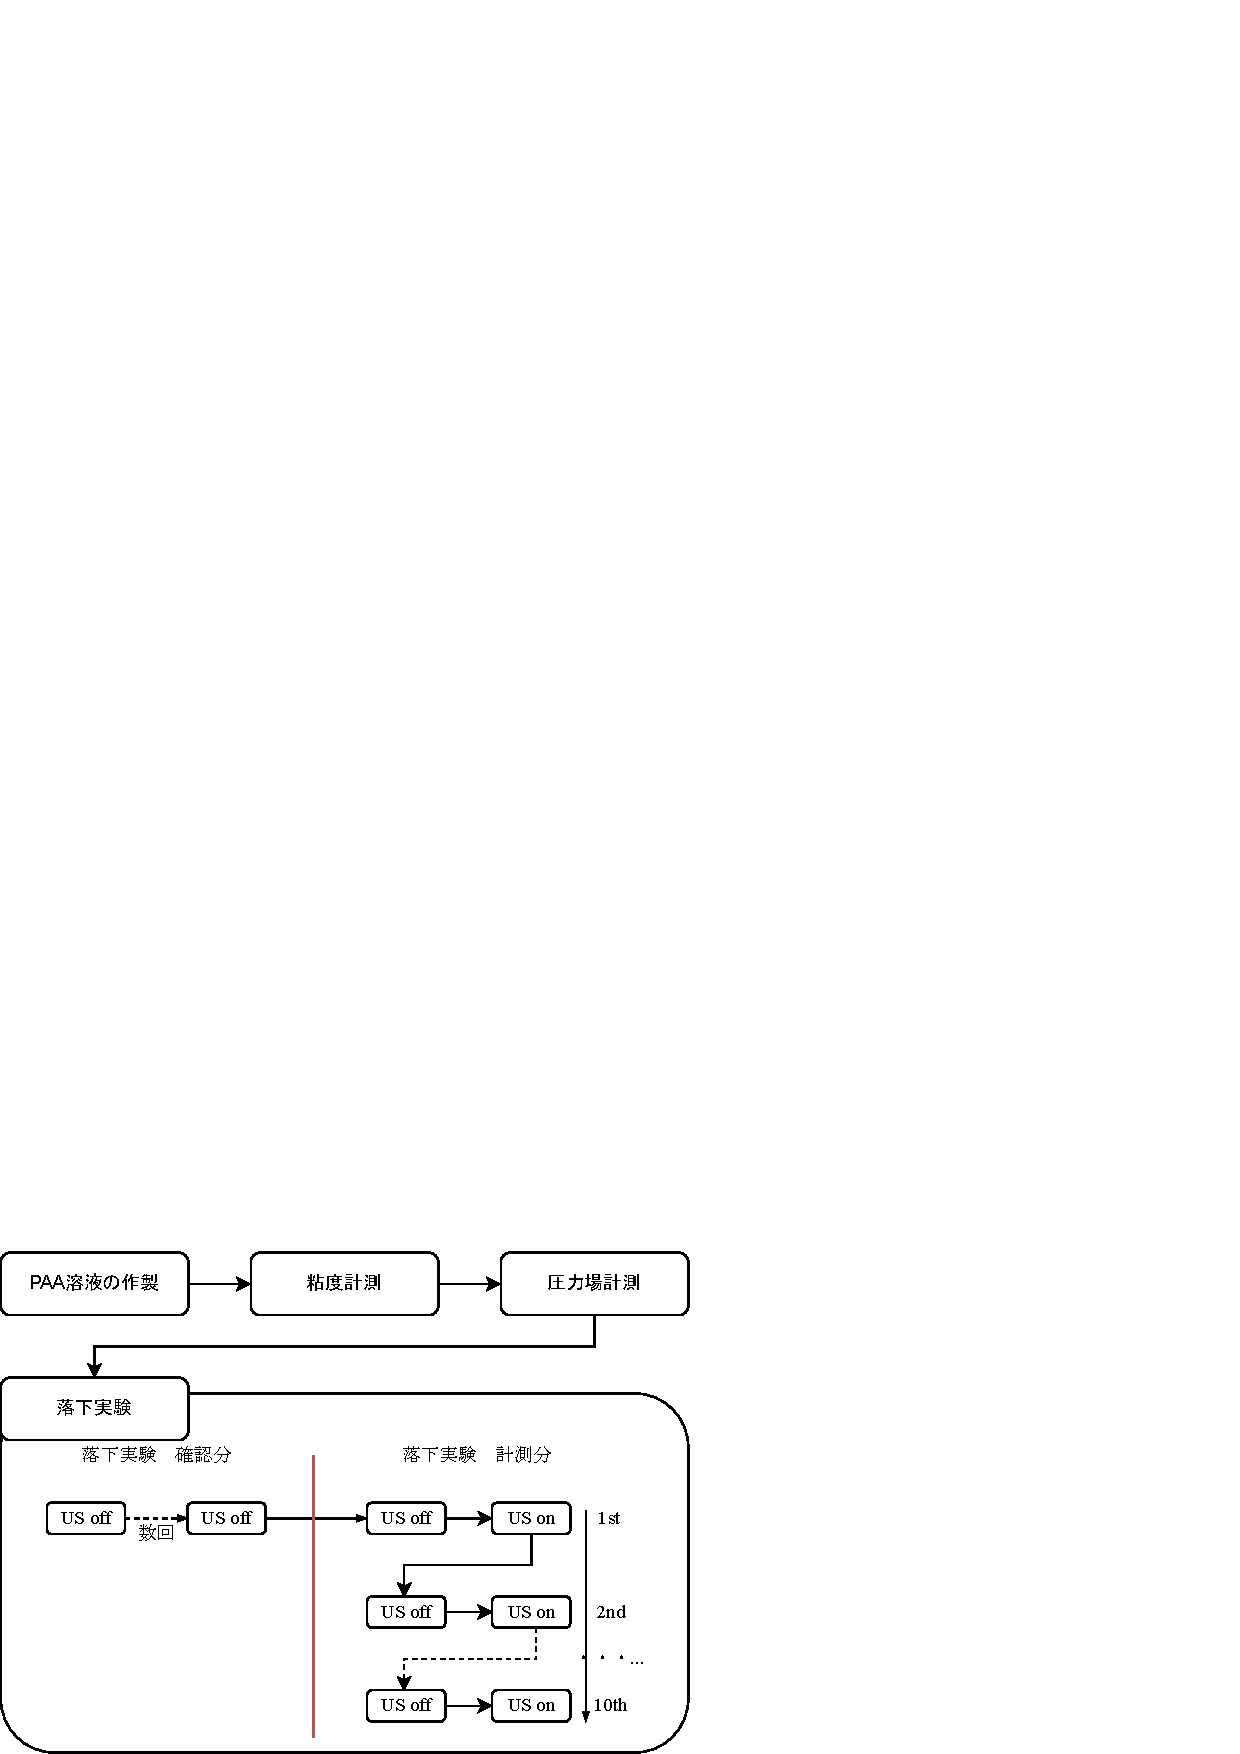
\includegraphics[clip,width=10.0cm]{2-Methods/exp-methods.png}
    \caption{Flowchart of the experimental procedure.}
    \label{fig:exp-methods}
\end{figure}
